\documentclass[conference]{IEEEtran}
\IEEEoverridecommandlockouts

\usepackage{amsmath,amssymb}
\usepackage{booktabs}
\usepackage{graphicx}
\usepackage{url}
\usepackage{balance}
\usepackage[hidelinks]{hyperref}
\usepackage{microtype}

% All numeric values in this manuscript are generated from the frozen result
% tables by pipeline/make_tables.py.  None is typed by hand.
\newcommand{\PinCoreBalAccApt}{0.608}
\newcommand{\PinCoreBalAccWeb}{0.731}
\newcommand{\PinCoreFprApt}{0.0}
\newcommand{\PinCoreFprWeb}{0.0}
\newcommand{\PinCoreRecallApt}{0.217}
\newcommand{\PinCoreRecallWeb}{0.463}
\newcommand{\PinIpBalAccApt}{0.773}
\newcommand{\PinIpBalAccWeb}{0.779}
\newcommand{\PinIpFprApt}{15.0}
\newcommand{\PinIpFprWeb}{15.3}
\newcommand{\PinIpRecallApt}{0.695}
\newcommand{\PinIpRecallWeb}{0.711}
\newcommand{\PinTwentyFourBalAccApt}{0.724}
\newcommand{\PinTwentyFourBalAccWeb}{0.739}
\newcommand{\PinTwentyFourFprApt}{7.4}
\newcommand{\PinTwentyFourFprWeb}{7.4}
\newcommand{\PinTwentyFourRecallApt}{0.523}
\newcommand{\PinTwentyFourRecallWeb}{0.551}
\newcommand{\aucApt}{0.851}
\newcommand{\aucWeb}{0.884}
\newcommand{\calAlarmApt}{0.55}
\newcommand{\calAlarmWeb}{0.50}
\newcommand{\contentAucApt}{0.725}
\newcommand{\contentAucWeb}{0.604}
\newcommand{\contentFoneApt}{0.020}
\newcommand{\contentFoneWeb}{0.017}
\newcommand{\corpusAddrApt}{2,660}
\newcommand{\corpusAddrWeb}{1,753}
\newcommand{\corpusCoresApt}{22}
\newcommand{\corpusCoresWeb}{40}
\newcommand{\corpusReqApt}{51,462}
\newcommand{\corpusReqWeb}{10,000}
\newcommand{\corpusSessApt}{3,126}
\newcommand{\corpusSessWeb}{254}
\newcommand{\foneApt}{0.362}
\newcommand{\foneWeb}{0.497}
\newcommand{\fprAlphaFiveApt}{3.9}
\newcommand{\fprAlphaFiveWeb}{4.4}
\newcommand{\fprAlphaTwoApt}{1.4}
\newcommand{\fprAlphaTwoWeb}{1.5}
\newcommand{\fprApt}{0.56}
\newcommand{\fprWeb}{0.85}
\newcommand{\latApt}{2.5}
\newcommand{\latWeb}{1.4}
\newcommand{\margMaxApt}{0.729}
\newcommand{\margMaxFeatApt}{distinct paths}
\newcommand{\margMaxFeatWeb}{total bytes}
\newcommand{\margMaxWeb}{0.590}
\newcommand{\praucApt}{0.667}
\newcommand{\praucWeb}{0.742}
\newcommand{\precApt}{0.920}
\newcommand{\precWeb}{0.906}
\newcommand{\recAlphaFiveApt}{0.445}
\newcommand{\recAlphaFiveWeb}{0.646}
\newcommand{\recAlphaTwoApt}{0.304}
\newcommand{\recAlphaTwoWeb}{0.481}
\newcommand{\recLfiveConcurrentApt}{0.485}
\newcommand{\recLfiveConcurrentWeb}{0.891}
\newcommand{\recLfiveTakeoverApt}{0.001}
\newcommand{\recLfiveTakeoverWeb}{0.002}
\newcommand{\recLfourConcurrentApt}{0.007}
\newcommand{\recLfourConcurrentWeb}{0.015}
\newcommand{\recLfourTakeoverApt}{0.001}
\newcommand{\recLfourTakeoverWeb}{0.002}
\newcommand{\recLoneConcurrentApt}{0.718}
\newcommand{\recLoneConcurrentWeb}{0.700}
\newcommand{\recLoneTakeoverApt}{0.001}
\newcommand{\recLoneTakeoverWeb}{0.002}
\newcommand{\recLthreeConcurrentApt}{0.005}
\newcommand{\recLthreeConcurrentWeb}{0.015}
\newcommand{\recLthreeTakeoverApt}{0.001}
\newcommand{\recLthreeTakeoverWeb}{0.002}
\newcommand{\recLtwoConcurrentApt}{0.405}
\newcommand{\recLtwoConcurrentWeb}{0.886}
\newcommand{\recLtwoTakeoverApt}{0.001}
\newcommand{\recLtwoTakeoverWeb}{0.173}
\newcommand{\recLzeroConcurrentApt}{0.893}
\newcommand{\recLzeroConcurrentWeb}{0.993}
\newcommand{\recLzeroTakeoverApt}{0.405}
\newcommand{\recLzeroTakeoverWeb}{0.882}
\newcommand{\recallApt}{0.229}
\newcommand{\recallHiApt}{0.247}
\newcommand{\recallHiWeb}{0.407}
\newcommand{\recallLoApt}{0.211}
\newcommand{\recallLoWeb}{0.311}
\newcommand{\recallWeb}{0.358}
\newcommand{\stateKBApt}{3.3}
\newcommand{\stateKBWeb}{4.6}
\newcommand{\tputApt}{52}
\newcommand{\tputWeb}{59}
\newcommand{\usMedApt}{17}
\newcommand{\usMedWeb}{16}
\newcommand{\usPnnApt}{52}
\newcommand{\usPnnWeb}{48}

% LaTeX's \input{} expands to \@@input<file>\relax.  Inside a tabular that
% trailing \relax lands at the start of the row following the body's last
% \\, which opens a cell and makes the next \bottomrule an illegal \noalign
% ("Misplaced \noalign").  \tabbody reads the file with no trailing token, so
% \bottomrule still sees the start of a row.  Used for table bodies only;
% tables/numbers above is read in the preamble and needs no such care.
\makeatletter
\newcommand{\tabbody}[1]{\@@input #1 }
\makeatother

\begin{document}

\title{Session-Continuity Invariants for Server-Side Detection\\ of HTTP Session Hijacking}

\author{\IEEEauthorblockN{Author names withheld for review}
\IEEEauthorblockA{Affiliation withheld for review}}

\maketitle

\begin{abstract}
A session identifier is a bearer credential: whoever presents it is served.
When one is stolen and replayed, the server sees a valid session, and the only
evidence that anything is wrong lies in how the session's observable client
context changes over time.  Cryptographic binding removes the problem but
requires client and ecosystem changes that most deployments do not have;
what deployments do instead is pin the session to an address or a
\texttt{User-Agent} string, a rule with no adjustable operating point whose
false-alarm rate is simply the rate at which legitimate clients move.  We
present SICA, a stateful, non-learning monitor that evaluates three graded
\emph{continuity invariants} per request against a pinned client binding, with
$O(1)$ time and fixed state per session.  Its organising idea is an asymmetry in
the \emph{shape} of a binding change rather than its magnitude: legitimate
mobility produces a monotone transition between bindings, whereas a live hijack
produces an interleaving that monotone mobility cannot.  SICA exploits it
twice --- the reference binding re-pins after a monotone transition but never
after a revisit, and an explicit fork invariant marks the revisit --- and we
report which of the two does the work.  Weights and the alerting threshold are
derived from attack-free traffic alone, so an operator specifies a false-alarm
budget in advance, something pinning rules structurally cannot offer.  We
evaluate on two public sample access-log corpora using a construction in which every
attacker request is a real request issued by a different real client of the same
server, so that no per-session summary feature separates the classes (largest
single-feature AUC \margMaxWeb\ and \margMaxApt; a one-class detector over all
eight such features reaches $F_1$ \contentFoneWeb\ and \contentFoneApt).  At a
$1\%$ budget SICA attains recall \recallWeb\ and \recallApt\ at measured
false-alarm rates of \fprWeb\% and \fprApt\%, with ROC AUC \aucWeb\ and
\aucApt, alerting a median of \latWeb\ attacker requests after the theft.
Detection is near-complete against an off-network adversary and falls to the
noise floor against one that reproduces the victim's subnet \emph{and} agent; we
report that boundary rather than averaging across it.  Two cells sharpen it: an
agent-cloning attacker is caught almost always when the victim keeps browsing and
almost never when the victim stops, and an attacker at the victim's own address
who merely runs a different client program is still caught
\recLfiveConcurrentWeb\ of the time while the victim browses --- so what the
evidence requires is a binding inconsistency, not an address change.  Almost every false
alarm we observe comes from one phenomenon --- a client whose binding moves
across \texttt{/16} boundaries mid-session, overwhelmingly transient interface
flapping --- and none at all from the pooled unmodified real sessions of either
corpus.
\end{abstract}

\begin{IEEEkeywords}
session hijacking, session management, bearer tokens, anomaly detection,
false-alarm budget, web security
\end{IEEEkeywords}

\section{Introduction}

HTTP is stateless, so applications carry authentication state in a session
identifier that the client returns with every request.  The identifier is a
\emph{bearer} credential: the server honours whoever presents it, and RFC 6265
notes plainly that transport encryption alone does not prevent an attacker from
obtaining one~\cite{rfc6265}.  Once an identifier leaks --- through a
cross-site scripting flaw, a mishandled log, a malicious extension, a shared
device, or an interception path --- the attacker is inside an authenticated
session that the application has no cryptographic reason to doubt.  Measurement
work has repeatedly found such identifiers exposed at scale on real
sites~\cite{sivakorn2016cookie}, and systematisations of web session security
treat post-authentication misuse as a first-class threat distinct from
credential compromise~\cite{calzavara2017surviving,calzavara2019subsession}.

The principled fix is to stop issuing bearer credentials.  Token
Binding~\cite{rfc8471} ties a token to a TLS-level key pair, and DPoP binds an
OAuth token to a client-held key with a per-request
proof~\cite{rfc9449}.  Both make a stolen identifier useless.  Both also
require the client, the application, and often intermediaries to change
together, which is why the overwhelming majority of deployed web sessions are
still bearer sessions.

What those deployments do instead is much cruder: they \emph{pin} the session.
On the first request the server records the client's address, or its
\texttt{User-Agent} string, or both, and terminates the session if the recorded
value ever changes.  Pinning is attractive because it is a one-line rule with a
clear rationale.  It has one structural defect that no amount of tuning fixes:
it has no operating point.  A pinning rule fires on every change, so its
false-alarm rate is exactly the rate at which legitimate clients change the
pinned attribute, and that rate is not small.  Addresses change mid-session
because of DHCP lease renewal, carrier-grade NAT pool rotation, and movement
between access networks~\cite{padmanabhan2016dynamic,richter2016cgn}; agent
strings change because browsers update.  An operator who needs a $1\%$
false-alarm budget cannot ask a pinning rule for one.

A second body of work evaluates client context statistically, but at the wrong
moment.  Risk-based authentication scores a \emph{login} against a user's
history of addresses and agents~\cite{freeman2016whoareyou,wiefling2019rba},
and is widely deployed for that purpose.  It says nothing about a session that
has already authenticated and is subsequently taken over, which is precisely the
hijacking case.  Continuous verification is an architectural goal of zero-trust
designs~\cite{nist2020zerotrust} but is usually left unspecified in mechanism.
Fingerprint-based session hardening has been proposed~\cite{unger2013shpf}, yet
fingerprints themselves evolve~\cite{vastel2018fpstalker,laperdrix2020survey},
so a rule that treats any fingerprint change as an attack inherits the same
defect as address pinning.

This paper asks a narrower question than "can we detect account takeover'': \emph{
given only what a server already logs, how much of an intra-session hijack is
observable, and can that evidence be delivered at a false-alarm rate the
operator chooses in advance?}  Our answer rests on one observation about the
shape of the evidence rather than its magnitude.  A legitimate client that moves
network or updates its browser produces a \emph{monotone} transition: it uses
binding $A$, then binding $B$, and never returns to $A$.  An attacker replaying
a stolen identifier while the victim is still browsing produces an
\emph{interleaving}: $A$, $B$, $A$, $B$.  Monotone mobility cannot manufacture an
interleaving, and a live hijack cannot avoid one.  That asymmetry is what
separates the two populations that pinning rules conflate.

\medskip\noindent\textbf{Contributions.}
\begin{enumerate}
\item \emph{Method.}  SICA, a stateful per-request monitor built from three
graded continuity invariants over a pinned client binding, in which the
monotone/interleaved asymmetry is realised both by a reference-migration policy
--- a legitimate move is charged once rather than for the remainder of the
session --- and by an explicit fork invariant.  It uses no learned component,
runs in $O(1)$ time per request, and holds fixed state per live session
(Section~\ref{sec:method}).
\item \emph{Budget-calibrated operation.}  A label-free calibration procedure
--- an applicability gate, benign-rarity weights, and a discrete budgeted
threshold over attack-free traffic --- that lets an operator specify a
session-level false-alarm budget in advance.  Against a nominal $1\%$ budget the
realised session-level false-alarm rates are \fprWeb\% and \fprApt\%, both
below the budget rather than merely near it (Section~\ref{sec:calibration}).
\item \emph{A benchmark that resists the shortcut.}  A construction on real
access logs in which every attacker request is a real request issued by a
different real client of the same server, length-matched to the victim session,
so that no per-session summary feature carries the label; and, symmetrically, an
explicit model of \emph{legitimate} mobility in the negative class, without
which a continuity detector cannot be evaluated at all
(Section~\ref{sec:benchmark}).
\item \emph{A detectability envelope rather than an average.}  Recall is
reported per adversary capability across a six-level masquerade ladder --- four
address-visible levels and two co-located levels in which the attacker presents
the victim's own address --- so the boundary at which server-side continuity
evidence disappears is stated instead of being averaged away
(Section~\ref{sec:envelope}).
\item \emph{A quantitative account of when pinning is viable.}  We locate the
benign-mobility rate at which address pinning ceases to be preferable, giving
operators a decision rule rather than a ranking (Section~\ref{sec:crossover}).
\end{enumerate}

\section{Threat Model}
\label{sec:threat}

\noindent\textbf{Terminology.}  We address \emph{session hijacking}: the use of
a valid, already-authenticated session identifier by a party other than the one
that authenticated.  We do not address session \emph{fixation} (the attacker
plants an identifier before authentication), credential theft (the attacker
learns the password and authenticates in their own right), or session
\emph{replay} of a completed transaction.  Those have different observables and
different defences.

\noindent\textbf{Legitimate user.}  Authenticates once and then issues a stream
of requests.  During the session the client may change its network address, at
any of three granularities, and may update its browser.  It may transiently
alternate between two network interfaces during a handover.  It cannot be in two
places at once for an extended period.

\noindent\textbf{Attacker.}  Has obtained a valid session identifier by some
means outside this model, and replays it from a client under their control.
The attacker chooses their own network position and may forge any
client-supplied header, including \texttt{User-Agent}.  The attacker cannot
compromise the server, cannot make the victim's client emit their requests, and
cannot rewrite the log.

\noindent\textbf{Server.}  Sees only what it already records for every request:
the remote address, the request line, the response status and size, the
timestamp, and the \texttt{User-Agent} and \texttt{Referer} headers.  It does
not see TLS key material, client-side telemetry, or geolocation.  It knows
which session identifier accompanied each request.

\noindent\textbf{Adversary capability ladder.}  The attacker's power is
parameterised by how much of the victim's binding they reproduce:

\smallskip
\noindent\begin{tabular}{@{}l@{\quad}p{0.78\columnwidth}@{}}
\texttt{L0} & own address (different \texttt{/16}), own agent\\
\texttt{L1} & own address (different \texttt{/16}), victim's agent\\
\texttt{L2} & address in victim's \texttt{/16}, different \texttt{/24}; own agent\\
\texttt{L3} & address in victim's \texttt{/24}; victim's agent\\
\texttt{L4} & victim's own address (shared NAT or proxy); victim's agent\\
\texttt{L5} & victim's own address; a different client program's own agent\\
\end{tabular}
\smallskip

\noindent and by whether the victim keeps using the session
(\emph{concurrent}) or stops (\emph{takeover}).  All six levels are evaluated
and reported.  \texttt{L0}--\texttt{L3} are \emph{address-visible}: the attacker
occupies a different address from the victim, so an address-change rule can in
principle see them.  \texttt{L4} and \texttt{L5} are \emph{co-located} --- the
attacker presents the victim's own address --- and they are not equivalent.  At
\texttt{L4} the attacker also reproduces the victim's agent, so the two bindings
are identical and \emph{no} binding signal exists; we make no claim of
protection against it and report it rather than excluding it.  At \texttt{L5} the
attacker is equally co-located but runs its own client program, so there is no
\emph{address} signal while $v_1$ still has evidence to read.  Retaining both is
deliberate: an envelope restricted to \texttt{L0}--\texttt{L3} would hand any
address-pinning rule perfect recall by construction and reduce the benchmark to
address-change detection.  We make no claim against an attacker content to issue
a single request.

\section{Method}
\label{sec:method}

\begin{figure*}[t]
\centering
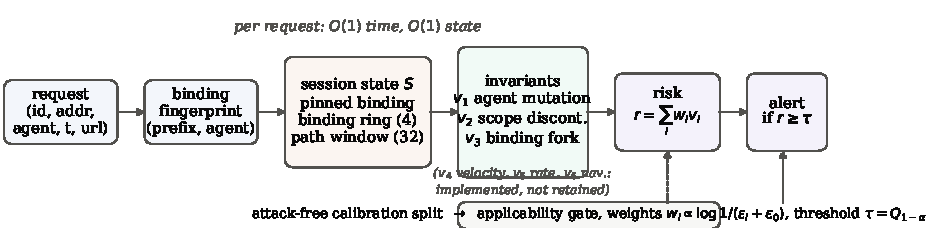
\includegraphics[width=\textwidth]{../results/figures/fig1_architecture.pdf}
\caption{SICA processing path.  Each request is reduced to a client binding and
compared against the session's pinned reference and bounded history; the
invariant vector is combined into a risk score and thresholded.  Weights and
threshold come from attack-free calibration traffic and are frozen before any
evaluation session is scored.}
\label{fig:arch}
\end{figure*}

\subsection{Bindings and session state}

For each request the monitor derives a \emph{binding}
$b=(a,\,p_{24},\,s_{16},\,\beta,\,\nu,\,\omega,\,\delta)$ comprising the remote
address $a$, its \texttt{/24} prefix $p_{24}$ and \texttt{/16} scope $s_{16}$,
and a fixed-rule parse of the \texttt{User-Agent} into browser family $\beta$,
major version $\nu$, operating-system family $\omega$ and device class $\delta$.
The \emph{core} agent identity $(\beta,\omega,\delta)$ is kept separate from the
version so that a browser upgrade and a browser substitution can be scored
differently.  An absent or unparseable agent maps to an explicit
\texttt{unknown} identity rather than to a missing value, so that an agent
disappearing mid-session is itself observable.

Fig.~\ref{fig:arch} shows the processing path.
Per live session the monitor holds: the pinned reference binding, the identity
of the most recent binding, a bounded ring of the last $m=4$ distinct binding
identities, a bounded window of the last $P=32$ in-session URLs, an
exponentially weighted inter-arrival gap, the request count and the running peak
risk.  Every field is fixed-width or bounded, so state is $O(1)$ per session and
the work done per request is a fixed number of comparisons.

\subsection{Continuity invariants}

Each invariant maps a request and the session state to a violation degree in
$[0,1]$; zero means "consistent with an uninterrupted single-client session''.
Grading is not cosmetic --- an ungraded rule inherits the rate of its most
common benign cause as its false-alarm rate, which is exactly the pinning defect.

\emph{$v_1$, agent mutation.}  $1$ if the core agent identity differs from the
pinned one, $0.35$ if only the major version differs, else $0$.  A browser does
not change family, operating system or device class between two requests of one
session; a version change is possible in principle and is therefore weak rather
than zero evidence.

\emph{$v_2$, network-scope discontinuity.}  $1$ if the \texttt{/16} differs from
the pinned scope, $0.45$ if the \texttt{/24} differs, $0.15$ if only the address
differs, else $0$.  The three levels correspond to leaving the administrative
network, changing access network, and a lease renewal or NAT pool rotation ---
respectively rare, occasional and routine~\cite{padmanabhan2016dynamic,richter2016cgn}.

\emph{$v_3$, binding fork.}  $1$ if the current binding was seen earlier in this
session but is not the immediately preceding one, else $0$.  This is the
discriminating invariant.  A roaming client abandons its old binding, producing
$A\,A\,B\,B$; concurrent use of one identifier from two clients produces
$A\,B\,A\,B$, and only the latter contains a revisit (Fig.~\ref{fig:mech}).

These three are the retained set.  Section~\ref{sec:rejected} reports three
further invariants that were implemented, evaluated and not retained.

\begin{figure}[t]
\centering
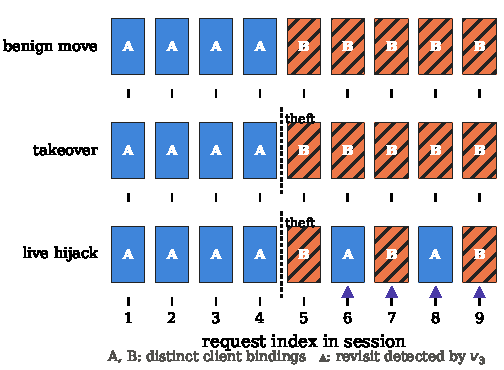
\includegraphics[width=\columnwidth]{../results/figures/fig2_mechanism.pdf}
\caption{Why the fork invariant separates what pinning conflates.  A benign
move and a silent takeover both produce a single monotone transition and are
therefore indistinguishable from server-side continuity alone.  A live hijack,
in which the victim keeps browsing, necessarily interleaves two bindings, and
the revisits ($\blacktriangle$) have no single-client explanation.}
\label{fig:mech}
\end{figure}

\subsection{Three invariants we implemented and rejected}
\label{sec:rejected}

Three further invariants suggested themselves and were implemented.  $v_4$, a
transition-velocity check firing when a network-scope change occurs faster than
association and routing could plausibly settle.  $v_5$, a rate-discontinuity
check firing when the inter-arrival gap collapses relative to the session's own
smoothed cadence.  $v_6$, a navigation-context break firing when a request
carries a first-party \texttt{Referer} naming a page the session has not
retrieved.  All three are reasonable, and none is retained.

The set was fixed on a \emph{development} seed block disjoint from every seed
used for a reported result.  This is a weaker form of independence than a
held-out corpus and we do not claim otherwise: the development seeds draw
different injections and different churn over the \emph{same} benign sessions,
so they control for the benchmark draw but not for the corpus.  The criterion was
declared in advance:
threshold-free ranking quality (ROC AUC), required to agree across both
workloads.  Ranking quality rather than $F_1$ or the realised false-alarm rate,
because the operating point is a separate, operator-chosen parameter; comparing
candidate sets at a nominal budget that each misses by a different margin would
confound the choice of invariants with the choice of threshold.

The reasons the three fail are specific rather than incidental.  In a log
without geographic coordinates, $v_4$ fires on the same event $v_2$ already
reports, double-counting one piece of evidence.  $v_5$ cannot be evaluated at
all on these corpora, and the reason lies in the source logs rather than in the
invariant: the upstream minute field is constant in W1 and takes two values in
W2, so no session spans more than $59$\,s and every inter-arrival gap is an
artefact of whatever produced the timestamps rather than a record of client
cadence.  A rate-discontinuity check reads exactly that quantity.  We therefore
reject $v_5$ as unevaluable here, and make no claim in either direction about the
signal it would carry on traffic with genuine timestamps.  $v_6$ reduced ranking quality on the one workload
where it is applicable at all, and is inapplicable on the other; dropping it
also removes the only corpus-level parameter (the first-party host set) from the
deployed configuration.

All three remain in the released implementation, and
Section~\ref{sec:ablation} reports restoring each of them to the retained set,
so the rejections are auditable rather than asserted.  One consequence is worth
stating plainly: the retained set reads no inter-arrival gap, no byte count, no
request count, no session duration and no request path.  Any residual marginal
signal in those quantities therefore cannot reach the detector, whatever the
benchmark construction did to them.

\subsection{Reference migration}

The reference binding is re-pinned after a \emph{monotone} transition and never
after a revisit.  Without migration, a client that legitimately moves is charged
$v_1$ and $v_2$ on every remaining request of its session, so the false-alarm
cost of a single move grows with session length.  With migration a move is
charged once.  A silent takeover is likewise charged once, which is the correct
consequence: as Fig.~\ref{fig:mech} shows, a takeover and a legitimate move are
the same event as far as continuity evidence is concerned.

The second half of the policy is the load-bearing one.  A revisit never re-pins,
because when two bindings are interleaved there is no basis for deciding which is
the owner --- so during a concurrent hijack the reference stays put and $v_1$ and
$v_2$ continue to fire on every request from the other binding.  The
monotone/interleaved asymmetry is therefore expressed twice in the design: once
in the migration policy, and once explicitly in $v_3$.  They are not redundant,
but they are not independent either, and Section~\ref{sec:ablation} reports how
much each contributes rather than leaving the reader to assume it is the
explicit one.

\subsection{Risk and label-free calibration}
\label{sec:calibration}

The per-request risk is the weighted sum $r=\sum_i w_i v_i$, and a session's
score is its peak per-request risk.  Both the weights and the alerting threshold
are derived from an attack-free calibration partition, in three steps.

\emph{Applicability gate.}  An invariant whose precondition is never exercised
in a deployment --- a referrer rule on traffic that carries no referrers --- is
not a strong invariant that happens never to fire; it is one that cannot fire.
Let $\pi_i$ be the fraction of calibration requests in which invariant $i$'s
precondition holds.  Invariants with $\pi_i<0.01$ are disabled and their weight
mass is redistributed.  Without this gate a rarity prior awards an
unexercisable invariant the largest possible weight and dilutes every invariant
that is actually observable; in our second workload the gate correctly disables
$v_6$, whose applicability is $0$.

\emph{Benign-rarity weights.}  Let $\varepsilon_i$ be invariant $i$'s mean
violation degree over calibration requests.  Weights are proportional to the
self-information of the invariant firing under the benign model,
\begin{equation}
w_i \;\propto\; \log\!\big(1/(\varepsilon_i+\varepsilon_0)\big),
\qquad \varepsilon_0 = 0.01 ,
\end{equation}
normalised over the applicable set.  The logarithm is used rather than
$1/\varepsilon_i$ because the reciprocal is unbounded as $\varepsilon_i\to 0$
and lets one quiet invariant dominate.  No attack label enters this
computation.

\emph{Budgeted threshold.}  Given an operator's session-level false-alarm budget
$\alpha$, the threshold $\tau$ is the \emph{smallest observed calibration peak
risk whose in-sample alarm rate does not exceed} $\alpha$, computed through the
identical evidence pipeline that evaluation will use.  A quantile is not used and
would not be correct here: session peak risk is a heavily tied discrete quantity,
so a $(1-\alpha)$ quantile combined with a $\text{peak}\geq\tau$ decision admits
an entire tie group and overshoots the budget.  Selecting over the observed
values instead makes the in-sample guarantee exact by construction, and the
realised calibration alarm rates reported in Section~\ref{sec:eval} show that it
also transfers out of sample.  Calibrating on a different statistic than the one
deployed silently breaks the budget; we make the second calibration pass for
this reason.  $\tau$ is frozen before any evaluation session is scored, and
evaluation labels are read only to compute metrics after every decision exists.
This is the property whose absence is the standard source of optimistic
operating points in security evaluations~\cite{arp2022dosdonts}.

\subsection{Complexity}

Per request the monitor performs a bounded agent parse, three prefix
comparisons, a membership test in a ring of four, a membership test in a window
of $32$, and an EWMA update: $O(1)$ time, $O(1)$ state per live session, no
scan over session history and no cross-session structure.

\section{Benchmark Construction}
\label{sec:benchmark}

\subsection{Why the benchmark must be constructed}

No public corpus labels individual HTTP requests as belonging to a hijacked
session.  Hijacks are rare, the ground truth is normally unavailable even to the
operator, and publishing labelled session traffic is a privacy problem in
itself.  The attack condition must therefore be constructed --- which is
acceptable only if the construction does not smuggle the label into the data.
This is the failure mode that invalidates many semi-synthetic security
benchmarks~\cite{sommer2010closedworld,arp2022dosdonts,rossow2012prudent}, and
avoiding it is a design requirement, not an afterthought.

\subsection{Corpora and sessionisation}

We use two public sample access logs with disjoint client populations
(Table~\ref{tab:corpus}), both redistributed by the Elastic Examples repository
and verified byte-identical to their upstream copies: \textbf{W1}, Apache-logged
human web browsing, and \textbf{W2}, Nginx-logged traffic from
package-manager-style clients.  Neither is claimed to be production traffic, and
W2 in particular is a demonstration corpus: its URL universe is three placeholder
download paths, its $404$ rate is high, and it carries essentially no referrers.
The substrate is real observed traffic; this is not a real-world attack dataset,
and the attacks are constructed.
W2 is included precisely because it is adversarial to our method: its
\corpusCoresApt\ distinct agent cores across \corpusReqApt\ requests make
agent-based evidence nearly useless, testing whether the method degrades
gracefully when client diversity is low.

Requests are grouped into sessions by client identity with a $1800$\,s idle
timeout, following the standard convention in web-log
analysis~\cite{catledge1995browsing,cooley1999preparation}, and sessions shorter
than seven requests are discarded so that every retained session admits a theft
point.  Client identity is used only to construct ground truth --- it defines
which requests genuinely belong to one client.  The detector never sees it; it
sees only the session identifier.

\begin{table*}[t]
\caption{Public sample access-log corpora and the sessions derived from them.}
\label{tab:corpus}
\centering\footnotesize
\begin{tabular}{lrrrrrrrrrrr}
\toprule
& \multicolumn{6}{c}{Raw log} & \multicolumn{5}{c}{Sessions ($\geq 7$ requests, $1800$\,s idle)}\\
\cmidrule(lr){2-7}\cmidrule(lr){8-12}
Workload & Requests & Addresses & \texttt{/16}s & Agents & Agent cores & Referrers & Span (d) & Sessions & Requests & Median & p90\\
\midrule
\tabbody{tables/corpus}
\bottomrule
\end{tabular}
\end{table*}

\subsection{Attack injection}

A victim session is chosen, a theft point is drawn between $25\%$ and $50\%$ of
its length, and $k$ attacker requests are inserted.  Three properties make the
construction resistant to shortcut learning.

\emph{The attacker's requests are real.}  Each attacker request is taken
verbatim --- path, referrer, status, size, and recorded inter-arrival gap --- from
a \emph{different real client} of the same server.  The gap is copied for
completeness only: as Section~\ref{sec:rejected} notes, these corpora's
timestamps are degenerate, so no timing property of the construction is claimed
and the retained invariants read no clock.  Only the binding is
substituted, according to the masquerade level.  The attacker's marginal
distributions are therefore drawn from exactly the same population as the benign
traffic, and identical request content appears in both classes.

\emph{The construction is length-matched.}  Attacker requests \emph{replace} an
equal number of the victim's post-theft requests --- a takeover replaces the
tail, a concurrent hijack displaces a random subset of it --- so an injected
session contains exactly as many requests as the original.  Without this,
request count alone predicts the label and every detector inherits the artefact.

\emph{The negative class contains legitimate mobility.}  Grouping by client
identity gives clean ground truth but makes benign binding changes impossible by
construction, which would render a continuity detector's false-alarm rate
meaningless.  We therefore apply explicit benign churn to a declared share of
benign sessions: monotone address change at one of three granularities (rate
$0.15$; $50\%$ intra-\texttt{/24}, $30\%$ intra-\texttt{/16}, $20\%$
cross-scope), agent version upgrade, both together, and transient interface
flapping (rate $0.05$), the last being an \emph{interleaved} benign phenomenon
included deliberately because it is the one thing that mimics a live hijack.
The churn rates are assumptions, not measurements; each is swept in
Section~\ref{sec:robustness} and the corresponding results are reported as
curves.

\subsection{Protocol}

Sessions are split into a calibration and an evaluation partition, by default
temporally.  Attacks are injected only into evaluation sessions, so the
calibration partition is attack-free by construction.  Weights and threshold are
derived from calibration alone and frozen; evaluation sessions are then replayed
through the frozen monitor; labels are read only afterwards.  Every experiment
is repeated over $30$ independent draws of the construction (seeds
$0$--$29$).  Design choices --- the evidence rule, reference migration, and the
composition of the invariant set --- were settled on a \emph{disjoint}
development seed block ($100$--$119$) and not revisited.  Reporting and
development seeds are disjoint seed blocks over the same corpora, not independent
datasets.  Attack labels are evaluation-only: they enter neither the scoring, nor
the benign weighting, nor the threshold, and are read only to compute metrics
once every decision exists.

\section{Evaluation}
\label{sec:eval}

\subsection{Setup and metrics}

Unless stated otherwise the budget is $\alpha=0.01$, the attack rate is $20\%$
of evaluation sessions, and the adversary is drawn uniformly from the twelve
\texttt{L0}--\texttt{L5} $\times$ \{takeover, concurrent\} cells --- the
co-located levels included, which is why the aggregate recall below is far from
the \texttt{L0} figure.  The unit of
decision is the session, because an operator responds to a session.  We report
precision, recall, $F_1$, the measured false-alarm rate, ROC and PR AUC, and
detection latency in attacker requests.  The detector is deterministic given a
request stream, so the reported variability comes entirely from the benchmark
draw and the calibration split; intervals are percentile bootstrap over the
$30$ draws.

\subsection{Does the benchmark leak?}
\label{sec:leakage}

Table~\ref{tab:leakage} answers this first, because every later number depends
on it.  Each of eight per-session summary features that a conventional detector
would use is scored alone against the injected label.  The largest single-feature
AUC is \margMaxWeb\ on W1 (\margMaxFeatWeb) and \margMaxApt\ on W2
(\margMaxFeatApt).  Two qualifications are owed.  A ROC AUC below $0.5$ is not
chance but an inverted signal, and on W1 the median inter-arrival gap sits
further below $0.5$ than any feature sits above it; on W2 the distinct-path count
is a genuine residual shortcut, an artefact of that corpus's three-path
universe.  Neither can reach the proposed monitor, which reads no gap, no byte
count and no path (Section~\ref{sec:rejected}); they bound what a
\emph{feature-based} detector could claim on this benchmark, and we report them
rather than removing the features.  A deterministic one-class
detector fitted to all eight features on the attack-free calibration split and
thresholded at the same budget reaches ROC AUC \contentAucWeb\ and
\contentAucApt\ but only $F_1$ \contentFoneWeb\ and \contentFoneApt, because at
a $1\%$ budget it recovers almost nothing.  The information that identifies an
injected session is therefore not in the marginal features; it is in the
relationship between a request and the session it was inserted into.  The
proposed monitor consumes none of these features.

Table~\ref{tab:splits} rules out two further sources.  A client-disjoint split,
in which no client contributes sessions to both partitions, and a random split
agree with the temporal split, so neither client identity nor time ordering is
carrying the result.

\begin{table}[t]
\caption{Leakage audit: ROC AUC of each per-session summary feature alone
against the injected label. Chance is $0.5$.}
\label{tab:leakage}
\centering\footnotesize
\begin{tabular}{lrr}
\toprule
Feature & W1 web & W2 apt\\
\midrule
\tabbody{tables/leakage}
\bottomrule
\end{tabular}
\end{table}

\begin{table}[t]
\caption{Split sensitivity. Agreement across the three splits shows that
neither client identity nor time ordering carries the result.}
\label{tab:splits}
\centering\footnotesize
\begin{tabular}{lrrrrrr}
\toprule
& \multicolumn{3}{c}{W1 web} & \multicolumn{3}{c}{W2 apt}\\
\cmidrule(lr){2-4}\cmidrule(lr){5-7}
Split & Rec. & FAR & AUC & Rec. & FAR & AUC\\
\midrule
\tabbody{tables/splits}
\bottomrule
\end{tabular}
\end{table}

\subsection{Main result}

\begin{table*}[t]
\caption{Detection at the frozen, label-free operating point ($\alpha=0.01$),
over $30$ independent benchmark draws. Intervals are percentile bootstrap
$95\%$ CIs of the mean. Latency is the median number of attacker requests
observed before the alert.}
\label{tab:main}
\centering\footnotesize
\begin{tabular}{lrrrcrrcrrr}
\toprule
Workload & Attacks & Prec. & Recall & 95\% CI & $F_1$ & FAR & 95\% CI & ROC AUC & PR AUC & Latency\\
\midrule
\tabbody{tables/main}
\bottomrule
\end{tabular}
\end{table*}

Table~\ref{tab:main} gives the headline figures.  On W1 the monitor recovers
recall \recallWeb\ (CI $[\recallLoWeb, \recallHiWeb]$) at a measured false-alarm
rate of \fprWeb\%, with precision \precWeb\ and ROC AUC \aucWeb.  On W2 recall
is \recallApt\ at \fprApt\%, with ROC AUC \aucApt.  Both realised rates sit
below the nominal $1\%$ budget rather than at it, and the calibration
partition's own alarm rate is \calAlarmWeb\% and \calAlarmApt\% --- so the
budget transfers from calibration traffic to later traffic rather than being met
only in-sample.  We claim budget \emph{adherence}, not that the realised rate
equals $1\%$.  The
median alert arrives \latWeb\ and \latApt\ attacker requests after the theft,
which matters more operationally than the aggregate: an alert that arrives after
the attacker has finished is worth little.

\subsection{The detectability envelope}
\label{sec:envelope}

\begin{figure*}[t]
\centering
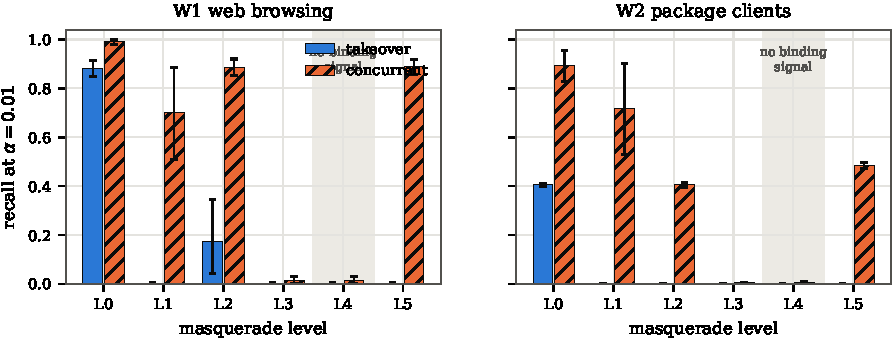
\includegraphics[width=\textwidth]{../results/figures/fig3_envelope.pdf}
\caption{Recall by adversary capability at $\alpha=0.01$, evaluated one cell at
a time. Detection falls as the attacker reproduces more of the victim's binding
and reaches the noise floor at \texttt{L3} and \texttt{L4}. The shaded column is
\texttt{L4}, the one cell in which attacker and victim bindings are identical so
that no binding signal exists at all. \texttt{L5} is equally co-located --- the
attacker again presents the victim's own address --- but runs a different client
program, leaving $v_1$ with evidence; it is detected whenever the victim keeps
browsing, and it is the cell that shows the method is not an address-change
detector. Bars show bootstrap $95\%$ CIs.}
\label{fig:envelope}
\end{figure*}

The aggregate in Table~\ref{tab:main} is an average over a uniform prior on
adversary capability, and a uniform prior is an arbitrary choice.
Table~\ref{tab:scenarios} and Fig.~\ref{fig:envelope} therefore report each cell
separately.  Against an off-network attacker using their own client
(\texttt{L0}) recall is \recLzeroConcurrentWeb\ (concurrent) and
\recLzeroTakeoverWeb\ (takeover) on W1.  At \texttt{L3}, where the attacker
sits in the victim's \texttt{/24} with the victim's agent, recall is
\recLthreeConcurrentWeb\ and \recLthreeTakeoverWeb\ --- effectively nothing.
\texttt{L4} is at the same floor (\recLfourConcurrentWeb\ and
\recLfourTakeoverWeb\ on W1), and there it is a floor by construction rather
than a limitation of the implementation: attacker and victim present the same
binding, so there is nothing for any binding-based rule to read.

\texttt{L5} is the cell that prevents this from being read as a story about
addresses.  The attacker is exactly as co-located as at \texttt{L4} --- the
victim's own address --- but issues requests from a different client program, so
no address evidence exists and $v_1$ carries the whole burden.  Recall is
\recLfiveConcurrentWeb\ on W1 and \recLfiveConcurrentApt\ on W2 when the
victim keeps browsing, against \recLfiveTakeoverWeb\ and \recLfiveTakeoverApt\
when the victim stops.  Two things follow.  The method detects hijacking with no
address signal whatsoever, which no address-pinning rule can do at any operating
point; and the detectable half is again the concurrent half, because a silent
takeover by a different client is a single monotone agent change, which is what a
legitimate device switch also looks like.  We claim this for the co-located
different-client case specifically, not for co-located attackers in general:
\texttt{L4} remains undetectable.

The informative comparison is not down the ladder but across it.  At
\texttt{L1} the attacker has cloned the victim's agent and differs only in
network, and the two modes diverge sharply: \recLoneConcurrentWeb\ against
\recLoneTakeoverWeb\ on W1, and \recLoneConcurrentApt\ against
\recLoneTakeoverApt\ on W2.  The attacker is identical in both cells; the only
difference is whether the victim keeps browsing.  That gap is the
monotone/interleaved asymmetry measured in isolation, and it is the clearest
evidence in the paper that the effect is real rather than an artefact of the
binding comparison.

We regard this degradation as the substantive finding rather than as a
weakness to be averaged away.  It says that server-side continuity evidence is
a function of how far the attacker is from the victim in binding space, and it
identifies exactly where the technique stops: an adversary who is co-located
with the victim and clones the agent is invisible to it, and defending against
that adversary requires cryptographic binding~\cite{rfc8471,rfc9449}, not better
heuristics.

\begin{table}[t]
\caption{Recall by masquerade level and concurrency, $\alpha=0.01$.}
\label{tab:scenarios}
\centering\footnotesize
\begin{tabular}{lrrrr}
\toprule
& \multicolumn{2}{c}{W1 web} & \multicolumn{2}{c}{W2 apt}\\
\cmidrule(lr){2-3}\cmidrule(lr){4-5}
Level & takeover & concurrent & takeover & concurrent\\
\midrule
\tabbody{tables/scenarios}
\bottomrule
\end{tabular}
\end{table}

\subsection{Where the false alarms come from}

\begin{table}[t]
\caption{False alarms attributed to the benign phenomenon that produced them,
pooled over $30$ draws. Sessions is the pooled count; FAR is a percentage.}
\label{tab:falsealarms}
\centering\footnotesize
\begin{tabular}{lrrrr}
\toprule
& \multicolumn{2}{c}{W1 web} & \multicolumn{2}{c}{W2 apt}\\
\cmidrule(lr){2-3}\cmidrule(lr){4-5}
Benign session class & Sess. & FAR & Sess. & FAR\\
\midrule
\tabbody{tables/false_alarms}
\bottomrule
\end{tabular}
\end{table}

Table~\ref{tab:falsealarms} attributes every false alarm to the legitimate
phenomenon that caused it, and the attribution is unusually clean.  Across all
pooled unmodified real sessions in both workloads, and across every session whose
only change was an agent upgrade or a monotone address change within the
\texttt{/24} or within the \texttt{/16}, the monitor raised \emph{no} false
alarm at all.  Almost every false alarm we observe comes from a client whose
binding crossed a \texttt{/16} boundary mid-session; the sole exception is a
small number of W1 sessions that flapped between two \texttt{/24}s inside one
\texttt{/16}, which is the same interleaving phenomenon one scale down.  The
highest rate by far is for the one benign phenomenon that structurally mimics a
hijack --- interface flapping across \texttt{/16}s, an interleaved binding change
with a single legitimate
owner.  This is the honest residual cost of the fork invariant, and it is
concentrated in a population an operator can reason about, rather than being
spread uniformly over ordinary users.

\subsection{Comparison with deployed rules}

\begin{table*}[t]
\caption{Comparison against deterministic non-learning baselines on identical
sessions and identical draws. Scored rules are calibrated to the same $1\%$
budget; pinning rules are parameter-free and are reported at whatever rate the
traffic produces. $^{\ast}$ marks a difference in $F_1$ against SICA that is
significant at $p<0.05$ (Wilcoxon signed-rank over $30$ paired draws, Holm-corrected).}
\label{tab:baselines}
\centering\footnotesize
\begin{tabular}{lrrrrrrrr}
\toprule
& \multicolumn{4}{c}{W1 web} & \multicolumn{4}{c}{W2 apt}\\
\cmidrule(lr){2-5}\cmidrule(lr){6-9}
Detector & Recall & FAR & Prec. & $F_1$ & Recall & FAR & Prec. & $F_1$\\
\midrule
\tabbody{tables/baselines}
\bottomrule
\end{tabular}
\end{table*}

\begin{figure*}[t]
\centering
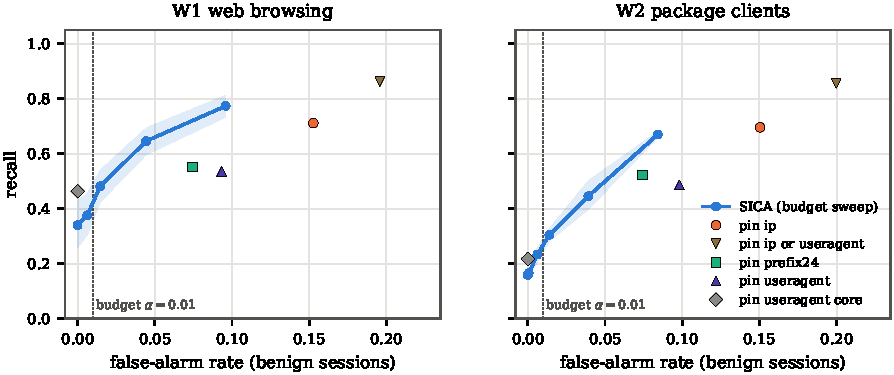
\includegraphics[width=\textwidth]{../results/figures/fig4_operating.pdf}
\caption{Operating characteristics. SICA traces a curve as the budget $\alpha$
is varied; each pinning rule is a single point, because it has no operating
parameter. In the low-false-alarm regime where a session detector is deployable,
the curve passes above the pinning points; address pinning is only preferable
once an operator will tolerate roughly a $15\%$ false-alarm rate.}
\label{fig:operating}
\end{figure*}

Table~\ref{tab:baselines} and Fig.~\ref{fig:operating} compare against the rules
that are actually deployed.  The comparison needs care, because $F_1$ at this
benchmark's $20\%$ attack prevalence rewards recall heavily and understates the
cost of false alarms.  Address pinning attains recall \PinIpRecallWeb\ on W1 and
\PinIpRecallApt\ on W2, at false-alarm rates of \PinIpFprWeb\% and
\PinIpFprApt\% --- an order of magnitude above the budget and, we would argue,
past the point of deployability.  Its recall is high because every attacker in
\texttt{L0}--\texttt{L3} changes address, and it is not higher because the two
co-located levels are inside the envelope: an address rule is blind to
\texttt{L4} and \texttt{L5} by construction.  This is the concrete payoff of not
restricting the ladder --- had we evaluated \texttt{L0}--\texttt{L3} only,
address pinning would have scored recall $1.0$ by construction and the
comparison would have carried no information.  Agent-core
pinning is a strong and nearly free rule on W1 (recall \PinCoreRecallWeb\ at
\PinCoreFprWeb\% measured false alarms) but is blind by construction to every
attacker that clones the agent, and collapses to \PinCoreRecallApt\ on W2 where
agent cores are near-uniform.

Two qualifications belong here rather than in a footnote.  First, agent-core
pinning measures $0\%$ false alarms because our benign model assigns zero
probability to a mid-session agent-core change; real causes exist (desktop-site
toggles, in-app browser hand-off, proxy rewriting), so that figure is an upper
bound on the baseline rather than a measurement.  Second, address pinning is a
parameter-free binary rule, so it has no ranking curve to compare: its single
operating point scores balanced accuracy \PinIpBalAccApt\ on W2, which is not
commensurable with SICA's ROC AUC of \aucApt.  What separates them is not ranking
quality but that SICA has an operating point and address pinning does not.  At
$\alpha=0.05$ SICA reaches recall \recAlphaFiveWeb\ at \fprAlphaFiveWeb\% ---
above \texttt{/24} pinning's \PinTwentyFourRecallWeb\ at
\PinTwentyFourFprWeb\% --- while at a $15\%$ false-alarm rate address pinning
remains ahead.  The claim we make is bounded accordingly: in the
low-false-alarm regime, graded continuity scoring dominates; in the
high-false-alarm regime it does not, and an operator who genuinely tolerates
$15\%$ session terminations should use address pinning.

\subsection{Precision at realistic base rates}

\begin{table}[t]
\caption{Precision and false-alert volume at deployment base rates, computed
from the measured true- and false-positive rates. Alerts are per million
sessions.}
\label{tab:baserate}
\centering\footnotesize
\begin{tabular}{lrrrr}
\toprule
& \multicolumn{2}{c}{W1 web} & \multicolumn{2}{c}{W2 apt}\\
\cmidrule(lr){2-3}\cmidrule(lr){4-5}
Hijack prevalence & Prec.\% & False alerts & Prec.\% & False alerts\\
\midrule
\tabbody{tables/base_rate}
\bottomrule
\end{tabular}
\end{table}

The precision in Table~\ref{tab:main} is measured at a $20\%$ attack prevalence
and does not transfer to deployment, where hijacked sessions are rare.
Table~\ref{tab:baserate} recomputes precision and alert volume from the measured
rates across realistic prevalences.  The base-rate arithmetic is
unforgiving~\cite{axelsson2000baserate}: at a prevalence of $10^{-3}$ the
monitor still emits far more false than true alerts, and the practical
consequence is that its output belongs in a graduated response --- step-up
authentication, re-authentication on the sensitive operation, analyst review ---
and not in an automatic termination.  We state this because the same arithmetic
disqualifies the pinning baselines far more sharply: at that prevalence address
pinning's \PinIpFprWeb\% false-alarm rate produces well over an order of
magnitude more alerts, for a recall gain that no analyst budget can absorb.  Alert volume, not
recall, is what determines whether a session detector survives contact with a
security operations centre~\cite{tariq2025alertfatigue}.

\subsection{Ablation and component selection}
\label{sec:ablation}

\begin{table}[t]
\caption{Leave-one-out over the three retained invariants (upper block) and
three design variants (lower block). $\Delta$ is relative to the full retained
method. Restorations of the rejected invariants are in the released ablation
table rather than here. $^{\ast}$: $p<0.05$, Wilcoxon signed-rank over $20$
paired draws, Holm-corrected.}
\label{tab:ablation}
\centering\scriptsize\setlength{\tabcolsep}{3.2pt}
\begin{tabular}{lrrrrrr}
\toprule
& \multicolumn{3}{c}{W1 web} & \multicolumn{3}{c}{W2 apt}\\
\cmidrule(lr){2-4}\cmidrule(lr){5-7}
Configuration & FAR & $\Delta F_1$ & $\Delta$AUC & FAR & $\Delta F_1$ & $\Delta$AUC\\
\midrule
\tabbody{tables/ablation}
\midrule
\tabbody{tables/design_ablation}
\bottomrule
\end{tabular}
\end{table}

\begin{figure}[t]
\centering
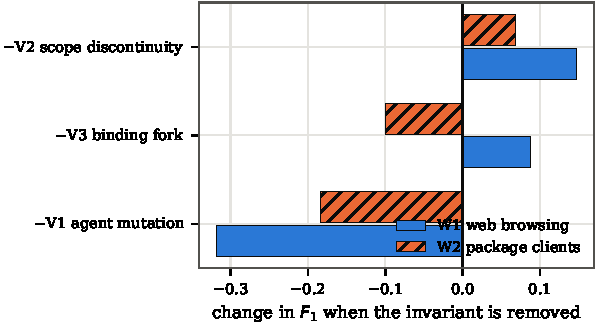
\includegraphics[width=\columnwidth]{../results/figures/fig6_ablation.pdf}
\caption{Change in $F_1$ when each retained invariant is removed and the
remainder is independently re-weighted and re-thresholded by the same
calibration procedure.}
\label{fig:ablation}
\end{figure}

Each ablation is separately and fully calibrated, so Table~\ref{tab:ablation}
and Fig.~\ref{fig:ablation} compare two independently configured detectors rather
than a detector against a de-tuned copy of itself.  Four things follow from it, and two of them cut
against the design.

\emph{The network-scope invariant carries the ranking.}  Removing $v_2$ costs
more ROC AUC than anything else in the table, on both workloads.  In the released
single-invariant configurations, $v_2$ alone also recovers most --- though not
all --- of the full method's ranking quality.  What it cannot do is operate: at
$\alpha=0.01$ a $v_2$-only detector raises no alert at all on either workload,
true or false, because a single graded invariant does not separate a calibration
tie group at that budget.  The ensemble's contribution is therefore not ranking
but the existence of a usable operating point.

\emph{The explicit fork invariant is not the decisive component.}  Removing it
lowers ROC AUC on both workloads, which is why the pre-declared selection
criterion retained it, but the effect is small and its $F_1$ effect does not even
share a sign: removing $v_3$ \emph{raises} $F_1$ on W1 and lowers it on W2.  At
the $\alpha=0.01$ operating point $v_3$ mostly trades recall for a lower
false-alarm rate rather than adding detections.  We report this rather than
presenting $v_3$ as the decisive component, because the aggregate does not
support that reading.

\emph{Reference migration is the larger expression of the same idea.}  Disabling
it costs more $F_1$ than removing any single retained invariant except $v_1$,
though it is not the most damaging row in the table: replacing the peak-risk
evidence rule with a decayed accumulator costs more still, on both workloads.
Since a revisit never re-pins, the migration policy already makes an interleaved
session score repeatedly through $v_1$ and $v_2$; $v_3$ marks the same event
explicitly and adds a smaller increment on top.  In ROC AUC the two are close
enough to be indistinguishable, so the claim we make is the $F_1$ one: the
monotone/interleaved asymmetry is doing the work the paper claims, but more
through the migration policy than through the invariant named after it.

\emph{Weighting and the rejected invariants.}  The uniform-weight control is
close to the benign-rarity weighting on these two workloads, so we do not claim
the weighting is decisive here; its role is to keep an invariant with a high
benign firing rate from dominating, which matters more as the invariant set
grows.  The released ablation additionally restores each rejected invariant to
the retained set.  Restoring $v_4$ or $v_5$ is measurably negative on both
workloads.  Restoring $v_6$ is not: it is inert on W2, where the applicability
gate disables it, and on W1 it \emph{raises} ROC AUC.  The rejection of $v_6$ was
made on the development seeds under the requirement that a candidate improve both
workloads, which $v_6$ cannot satisfy when it is unexercisable on one of them;
the reporting-seed ablation does not independently corroborate it, and we state
that rather than presenting the ablation as confirmation.

\subsection{Robustness to the benchmark's own assumptions}
\label{sec:robustness}
\label{sec:crossover}

\begin{figure*}[t]
\centering
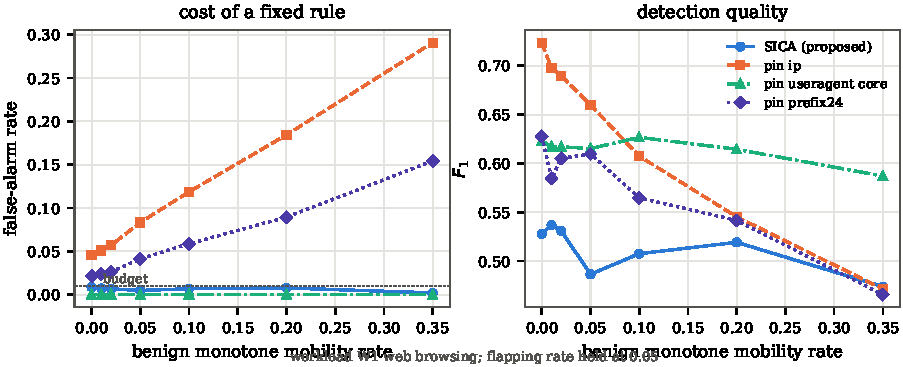
\includegraphics[width=\textwidth]{../results/figures/fig5_crossover.pdf}
\caption{When address pinning stops being viable. As benign mobility grows,
pinning's false-alarm rate rises with it because it has no operating point,
while the calibrated monitor holds its budget. The crossing point is the
quantity an operator needs in order to choose between them.}
\label{fig:crossover}
\end{figure*}

Several quantities in the benchmark are assumptions rather than measurements,
and a headline that depends on an unverifiable choice is not a result.  Each is
therefore swept.  The most consequential is the rate of benign mobility, and
Fig.~\ref{fig:crossover} shows why it decides the comparison rather than
decorating it: address pinning's false-alarm rate rises in lockstep with benign
mobility, because that rate \emph{is} its false-alarm rate, while the calibrated
monitor holds its budget across the sweep and pays instead in recall.  The
remaining sweeps --- flapping rate, attacker traffic volume, attack prevalence,
and minimum session length --- are reported in the released tables; the monitor's
false-alarm rate stays at budget throughout, and recall varies with the amount
of post-theft evidence available, as expected.

\subsection{Efficiency}

\begin{table}[t]
\caption{Measured cost, single-threaded, median of seven repetitions after two
warm-up runs. Throughput and latency are flat as the number of concurrently live
sessions grows by roughly $20\times$ within each workload, and across the two
workloads together the measured range spans from single-digit to four-figure
live sessions, as the $O(1)$ design requires.}
\label{tab:efficiency}
\centering\footnotesize\setlength{\tabcolsep}{3.2pt}
\begin{tabular}{lrrrrrr}
\toprule
Workload & Live sess. & Requests & kreq/s & $\mu$s med. & $\mu$s p99 & KiB/sess.\\
\midrule
\tabbody{tables/efficiency}
\bottomrule
\end{tabular}
\end{table}

Table~\ref{tab:efficiency} measures rather than asserts the lightweight claim.
A single unoptimised Python thread sustains \tputWeb\ and \tputApt\ thousand
requests per second, with a median per-request service time of \usMedWeb\ and
\usMedApt\,$\mu$s and a $99$th percentile of \usPnnWeb\ and \usPnnApt\,$\mu$s.
Measured state is \stateKBWeb\ and \stateKBApt\,KiB per live session.  Crucially,
all three quantities are flat as the number of concurrently live sessions grows:
by roughly $20\times$ within each workload's own scaling sweep, and over a much
wider span when the two sweeps are read together.  That flatness is the
observable consequence of the $O(1)$ design and the reason the measurement is
reported as a scaling table rather than a single number.  These are computational
costs measured on one machine; they are not detection delays, and no wall-clock
detection latency is claimed anywhere in this paper.

\section{Discussion and Limitations}

\noindent\textbf{What this cannot do.}  The envelope in
Section~\ref{sec:envelope} is the honest boundary.  An attacker who reproduces
the victim's \texttt{/24} and agent is invisible, and one who shares the victim's
address \emph{and} clones the agent (\texttt{L4}) is invisible to any
binding-based signal whatsoever.  Sharing the address alone is not sufficient for
that: at \texttt{L5} the same co-located attacker running a different client is
still caught while the victim browses.  A silent takeover is
information-theoretically the same event as a legitimate device change: both are
one monotone transition.  What remains detectable is the concurrent case --- which is also the common one
when a cookie is stolen from a user who is still browsing --- and there the
advantage is large: at \texttt{L1} the same attacker is caught
\recLoneConcurrentWeb\ of the time when the victim keeps browsing and
\recLoneTakeoverWeb\ of the time when the victim stops.  Nothing here substitutes for cryptographic
binding~\cite{rfc8471,rfc9449}; the method is for the large installed base that
does not have it.

\noindent\textbf{Threats to validity.}  The benign mobility model is the
principal one.  Its rates are declared assumptions and are swept, but its
\emph{shape} is ours: real clients may move in ways we did not model, and the
$0\%$ false-alarm rate we measure on unmodified sessions is partly a statement
about what our churn model does not generate.  In particular we assign zero
probability to a mid-session agent-core change, which flatters agent-core
pinning as well as our own $v_1$.  W1 is small --- \corpusSessWeb\ sessions ---
so its intervals are wide, and both logs are a decade old and neither carries
authentication.  Session identifiers are simulated by the ground-truth client
grouping; a deployment would use the real identifier, which is if anything
cleaner.  Finally, both corpora have degenerate timestamps --- a constant or near-constant
minute field --- so no session spans more than $59$\,s, every inter-arrival gap
is a generator artefact, and this benchmark can support no claim about timing,
session duration or client cadence.  The study survives that only because the
three retained invariants read no clock at all.  It does mean the rejected $v_5$
is unevaluable rather than refuted, and that the theft-delay sweep is an inert
condition here.

\noindent\textbf{Deployment.}  Alerts should drive graduated response, not
termination, for the base-rate reason above.  The monitor stores no content and
no cross-session state, and the pinned binding is derivable from data the server
already logs, so it adds no new personal data collection; the address prefixes
it retains are nonetheless personal data in most jurisdictions and should carry
the retention limits already applied to access logs.

\section{Conclusion}

Session hijacking is an intra-session continuity problem, and the shape of a
binding change --- monotone or interleaved --- carries information that its
magnitude does not.  Building a detector on that distinction, and calibrating it
on attack-free traffic alone, yields a monitor that tracks an operator-specified
false-alarm budget, alerts within a couple of attacker requests, costs
microseconds and kilobytes per session, and reports honestly the adversary at
which its evidence runs out.  The ablation locates the effect precisely: it lives
mostly in the policy of re-pinning the reference only on monotone transitions,
rather than in the invariant we named after it, and graded network evidence
alone already supplies most of the ranking quality.  Against deployed pinning rules the trade is
explicit rather than rhetorical: an order of magnitude fewer false alarms in
exchange for the detections that only an unbounded false-alarm rate can buy.

\balance
\bibliographystyle{IEEEtran}
\bibliography{ref}

\end{document}
